\documentclass[finnish]{tktltiki2}

% --- General packages ---

\usepackage[utf8]{inputenc}
\usepackage[T1]{fontenc}
\usepackage{lmodern}
\usepackage{microtype}
\usepackage{amsfonts,amsmath,amssymb,amsthm,booktabs,color,graphicx}
\usepackage[pdftex,hidelinks]{hyperref}
% Automatically set the PDF metadata fields
\makeatletter
\AtBeginDocument{\hypersetup{pdftitle = {\@title}, pdfauthor = {\@author}}}
\makeatother

% --- Language-related settings ---
%
% these should be modified according to your language

% babelbib for non-english bibliography using bibtex
\usepackage[fixlanguage]{babelbib}
\selectbiblanguage{finnish}

% add bibliography to the table of contents
\usepackage[nottoc]{tocbibind}
% tocbibind renames the bibliography, use the following to change it back
\settocbibname{Lähteet}

% --- Theorem environment definitions ---

\newtheorem{lau}{Lause}
\newtheorem{lem}[lau]{Lemma}
\newtheorem{kor}[lau]{Korollaari}

\theoremstyle{definition}
\newtheorem{maar}[lau]{Määritelmä}
\newtheorem{ong}{Ongelma}
\newtheorem{alg}[lau]{Algoritmi}
\newtheorem{esim}[lau]{Esimerkki}

\theoremstyle{remark}
\newtheorem*{huom}{Huomautus}


% --- tktltiki2 options ---
%
% The following commands define the information used to generate title and
% abstract pages. The following entries should be always specified:

\title{Rinnakkaisuus verkkopalvelinsovelluksessa}
\author{Vili Lipo}
\date{\today}
\level{Kanditaatin tutkielma}
\abstract{Tässä tutkielmassa vertaillaan verkkopalvelimien rinnakkaistamismalleja
  ja niiden suorituskykyä. Verkkopalvelin on ohjelma, joka vastaa useiden asiakkaiden pyyntöihin
  verkkosivuilla tai verkkosovelluksissa. Pyyntöihin vastaamiseen
  voi liittyä laskentaa, tietokantaoperaatioita tai muita toimenpiteitä.

Vertailuun valittiin tapahtumaohjattu Reactor-malli, SEDA-malli ja säiereservimalli}

% The following can be used to specify keywords and classification of the paper:

\keywords{avainsana 1, avainsana 2, avainsana 3}

% classification according to ACM Computing Classification System (http://www.acm.org/about/class/)
% This is probably mostly relevant for computer scientists
% uncomment the following; contents of \classification will be printed under the abstract with a title
% "ACM Computing Classification System (CCS):"
\classification{Software and its engineering $\rightarrow$ Software organization and properties
$\rightarrow$ Software system structures $\rightarrow$ Distributed systems organizing principles}

% If the automatic page number counting is not working as desired in your case,
% uncomment the following to manually set the number of pages displayed in the abstract page:
%
% \numberofpagesinformation{16 sivua + 10 sivua liitteissä}
%
% If you are not a computer scientist, you will want to uncomment the following by hand and specify
% your department, faculty and subject by hand:
%
% \faculty{Matemaattis-luonnontieteellinen}
% \department{Tietojenkäsittelytieteen laitos}
% \subject{Tietojenkäsittelytiede}
%
\begin{document}
\frontmatter      % roman page numbering for front matter

\maketitle        % title page
\makeabstract     % abstract page

\tableofcontents  % table of contents

% --- Main matter ---

\mainmatter       % clear page, start arabic page numbering

\section{Johdanto}
Verkkopalvelinsovelluksien suorituskyky vaikuttaa vahvasti
Internetin välityksellä käytettävien palveluiden käyttökokemukseen ja toimivuuteen.
Verkkopalvelimien taakat ovat vaihtelevia, ja tästä johtuen
yleispätevän verkkopalvelimen tulisi skaalautua saatavilla oleviin resursseihin.
Jos palvelimen käyttötarkoitus ei ole suorittaa pilvilaskentaa, sen
kriittisimmät resurssit ovat I/O-resurssit.
Verkkopalvelimen tehokkuuteen ja skaalautumiseen vaikuttaa olennaisesti
sen samanaikaistamiskäytäntö (concurrency policy). Tässä
tutkielmassa vertaillaan eri malleja palvelimen samanaikaistamiseen.

Verkkopalvelimien samanaikaistamismalli on osa sovellusta,
joka on mielekästä toteuttaa moduulina tai kirjastona.
Näin palvelimen sovelluslogiikka voidaan irrottaa rinnakkaisuutta
käsittelevästä logiikasta ja käyttää uudelleen toisissa projekteissa.

Vertailussa perehdytään Reactor-malliin ja sen jatkokehityksiin kuten Proactor-malliin,
sekä säiereservimalliin (threadpool-model).
Vertailun keskeisimmät kriteerit ovat suorituskyky, luotettavuus, ja
sovelluslogiikan kehittämiseen liittyvät haasteet.

Yksinkertaisuudestaan huolimatta tehokkailla asynkronisilla
kutsuilla varustettu Reactor-mallinen verkkopalvelinsovellus
kykenee vastaamaan suurenkin palvelun tarpeisiin, jos palvelun
pullonkaula on I/O-operaatiot.
Proactor-mallilla voidaan tuoda kehittäjille edistyneempiä työkaluja
asynkronisten kutsujen hallintaan.

Tarvittaessa järjestelmän voi laajentaa moniprosessimallia noudattavaksi,
jos tapahtumaohjatunjärjestelmän skaalautuvuus ei muuten riitä.

Säiereservimallin on hyvä vaihtoehto, jos palvelimen
toimintaan liittyy enemmän laskentaa ja sen huipputeho ei ole I/O-sidonnainen.
Laskennallisesti raskaaseen palvelimeen voidaan myös soveltaa SEDA-mallia.

Luvussa 2 kerrotaan taustatietota asiakas-palvelin mallista ja rinnakkaisuudesta sekä
esitellään verkkopalvelimien samanaikaistamismalleja. Luvussa 3
malleja vertaillaan ja analysoidaan. Luvussa 4 on yhteenveto aiheesta.
\section{Verkkopalvelinsovellus}
Verkkopalvelinsovellus on osa internetsivuston tai palvelun toteuttavaa
asiakas-palvelin järjestelmää. Tässä luvussa kerrataan
asiakas-palvelin malli ja rinnakkaisuuden keskeiset käsitteet.
Sen jälkeen käydään läpi eri malleja rinnakkaisuuden edistämiseen
verkkopalvelimissa. Erityisesti keskitytään I/O-operaatioiden suorittamiseen
samanaikaisesti.
\subsection{Asiakas-palvelin malli}
Asiakas-palvelin mallissa
asiakasohjelma tarjoaa käyttäjälle käyttöliittymän sovellukseen. Palvelinohjelma
tarjoaa määritellyn rajapinnan
palveluita asiakasohjelmalle verkkoyhteyden yli~\cite{sinha_client-server_1992}.
Tieto välittyy ohjelmien välillä pyyntöinä ja vastauksina ja näin palvelinohjelma ja
asiakasohjelma
muodostavat löysästi yhdistetyn järjestelmän.

Asiakasohjelma siis yhdistää käyttöliittymässä tapahtuvat toimet palvelimen
rajapinnan pyynnöiksi. Se voi hyödyntää pyyntöjen tulosten tallentamista
muistiin. Näin tarvittavia pyyntöjä voidaan vähentää, jos sen tulos
on jo paikallisessa muistissa. Asiakasohjelma voi myös suorittaa
laskentaa tai muita toimenpiteitä paikallisesti~\cite{sinha_client-server_1992}.

Asiakasohjelmat voivat olla työpöytäsovelluksia, jotka hyödyntävät käyttöjärjestelmän
ikkunointi-ja käyttöliittymäominaisuuksia~\cite{sinha_client-server_1992}.
Tämänkaltaisen asiakasohjelman toteuttamisessa voidaan käyttää mitä tahansa ohjelmointikieltä,
ja asiakasohjelman toiminnallisuutta voi laajentaa lähes rajatta.

Asiakasohjelma voi olla myös verkkosivu. 2000-luvun alussa
pelkkään staattiseen HTML-standardiin perustuvat verkkosivut pystyivät
tarjoamaan käyttöliittymiä esimerkiksi keskustelualustoille ja verkkokaupoille.
Näissä järjestelmissä valtaosa suorittamisesta on palvelimen vastuulla,
sillä sen pitää tiedonkäsittelemisen lisäksi kirjoittaa tieto
esitettävään HTML-muotoon käyttöliittymän näkymäksi. Palvelin
siis vastaa selaimen pyyntöön lähettämällä kokonaisen HTML-tiedoston.

Nykyisten selaimien JavaScript suoritustuen ansiosta yhä
monimutkaisempia asiakassovelluksia voidaan toteuttaa
selaimella saavutettavilla verkkosovelluksina.
Nykyään palvelimen ja asiakkaan
välisessä tiedonvälityksessä on muodikasta käyttää REST-rajapintaa, jossa
tieto on rakenteisessa muodossa. Asiakasohjelma tämän jälkeen piirtää siitä
itsenäisesti käyttöliittymän näkymän. [lähde?]

Palvelin tarjoaa sen rajapinnan määrittämiä palveluita asiakasohjelmille.
Palvelin ei itsenäisesti aloita yhteyttä mihinkään
asiakkaaseen vaan se odottaa niiden pyyntöjä.
Se pystyy palvelemaan useita asiakkaita, jopa
eri asiakasohjelmia, kunhan asiakasohjelmat noudattavat
palvelimen rajapintaa~\cite{sinha_client-server_1992}.

Palvelimen palvelut muodostavat järjestelmän keskeisen
sovelluslogiikan, jossa asiakaspyynnön parametreilla
suoritetaan toimintoja ja palvelin lähettää
tuloksen vastauksena~\cite{sinha_client-server_1992}.

Yleisesti palvelin vastaa järjestelmän turvallisuudesta sillä,
sen toiminnan vääristäminen on haastavampaa paha-aikeisille
toimijoille, kun taas asiakasohjelma toiminnan muuntelu, pyyntöjen
lähettäminen toisella ohjelmistolla on suoraviivaisempaa.

Asiakasohjelmaa ajetaan laitteella, joka ei ole verkkosovelluksen
ylläpitäjän hallussa. Paha-aikeiset toimijat voivat käyttää tätä hyväkseen
ja tarkkailla asiakasohjelman lähettämiä pyyntöjä tai sen
suorituskäyttäytymistä kuten resurssien käyttöä.
Tarkkailusta selvinneiden tietojen avulla on mahdollista
kiertää asiakasohjelmaan toteutettuja suojauksia.

Palvelinohjelman toimintaa vääristääkseen
paha-aikeisten toimijoiden tulisi päästä
käsiksi sitä suorittavan järjestelmän hallintatoimintoihin, tai
löytää haavoittuvuus sen rajapinnasta. Nämä hyökkäysvektorit
ovat huomattavasti kapeampia kuin sovelluksella jota
suoritetaan hyökkääjien omalla laitteistolla.
% etsi jokin tietoturvan perusteos
Palvelin vastaa myös tunnistautumisesta sekä käyttöoikeuksien hallinnasta.
Monen palvelun toteuttamisen kannalta on kriittistä, että
tiedon käyttöoikeuksia voidaan rajata käyttäjän tunnistautumisen perusteella.

Yksinkertainen esimerkki asiakas-palvelin mallista on tietokantapalvelin,
jossa tietokannan tiedot on tallennettu palvelimelle, josta voidaan
asiakasohjelmalla tehdä verkon yli tietokantakyselyitä.

Verkkopalvelin on palvelin, jonka tehtävä on vastata Internetin
sivuston tain palvelun toteuttamiseen
liittyviin pyyntöihin eli lähettämään tietyn HTTP-pyynnön
perusteella oikea HTML-tiedosto, tekstimuotoinen datatiedosto~\cite{Berners-Lee_1994}
,tai kuvatiedosto.
HTML-näkymät voivat olla valmiina tiedostojärjestelmässä tai
palvelin voi täydentää merkkauskielellä kirjoitettuun pohjaan
tietoja tietokannasta tai muusta sovelluksen tilatiedosta.
\subsection{Rinnakkaisuus palvelinsovelluksessa}

Rinnakkaisuudella tarkoitetaan tietojenkäsittelytieteessä useiden
eri operaatioiden suorittamista järjestelmässä samaan aikaan.
Nykyisissä palvelintietokoneissa on kymmeniä suorittimia ja niiden tehokkaaseen
hyödyntämiseen tarvitaan rinnakkaisuuden hallintaa.

On täysin ongelmakohtaista kuinka tehokkaasti se voidaan ratkaista rinnakkain.
Tähän vaikuttaa kuinka suuri osa tehtävästä on olemukseltaan peräkkäistä.
Peräkkäiset osat ovat sellaisia, jossa ohjelman vaiheet ovat täysin
riippuvaisia toisistaan ja seuraavaan vaiheeseen ei voida mennä ennen edellisen
valmistumista. Jos suuri osa ohjelmasta on peräkkäistä, ei rinnakaistamalla
saada hyötyä. Tällaisessa tapauksessa rinnakkaisuuden hallinnasta aiheutuvat
rasitteet saattavat jopa heikentää suorituskykyä~\cite{stallings_operating_2018}.

Riippumatta tehtävästä rinnakkaisuuden saavuttaminen on vaikeaa,
sillä se tuo ohjelmoijalle uusia haasteita, jotka eroavat tavallisesta
ohjelmoinnista. Ohjelmointivirheen riski on rinnakkaisissa osissa hyvin suuri,
koska ohjelman oikeellisuuden varmistaminen kaikissa mahdollisissa
suoritusjärjestyksissä on erittäin työlästä.
Keskeisiä ongelmia, joita rinnakkaisuus tuo ohjelmointiin on eri vaiheiden
synkronointi, tietorakenteiden suojaaminen ja lukkiutumisen hallinta.

Verkkopalvelinsovelluksessa yksi asiakkaan pyyntö HTTP-protokollan välityksellä
muodostaa mielekkään kokonaisuuden.
Järjestelmässä on toivottavaa, että pyyntöjä voitaisiin suorittaa
rinnakkain kaikilla järjestelmässä olevilla suorittimilla, tai muuten
saavuttaa korkea resurssien käyttöaste.
Näin ohjelmistojärjestelmä skaalautuu saatavilla oleviin resursseihin.
Käsiteltävät pyynnöt eivät yleisesti ole riippuvaisia
toisistaan ja niiden täyttäminen pääsääntöisesti vaatii I/O-laitteiden odottamista.
Näistä syistä verkkopalvelinsovellus on hyvä kohde rinnakkaistamiselle.

Yleisesti verkkopalvelimet toteutetaan käyttäen valmista sovelluskehystä eli kirjastoa,
joka toteuttaa palvelinmallin, ja tarjoaa rajapinnat sovelluslogiikan
kehittämistä varten. Tähän sovelluskehykseen on hyvä sijoittaa
palvelimen samanaikaisuuteen liittyvä logiikka.

Käyttöjärjestelmät tarjoavat kehittäjälle työkaluja, joilla rinnakkaisuuden hallintaan.
Niistä tärkeimpiä ovat prosessit ja säikeet.
Prosessi yksi ohjelma, joka on ajossa järjestelmässä. Sen suoritustilatiedot, ja tunniste on
tallennettu käyttöjärjestelmässä prosessin kuvaajaan~\cite{stallings_operating_2018}.
Jokaisella
prosessilla on oma muistialue, ja prosessien välinen keskustelu
tapahtuu ainoastaan käyttöjärjestelmän tarjoamien rajapintojen läpi~\cite{stallings_operating_2018}.
Prosessi siis käsitteenä mahdollistaa sen että, käyttöjärjestelmä
voi suorittaa useaa ohjelmaa samanaikaisesti ja käyttöjärjestelmän
vuoronantaja jakaa niille suoritusaikaa. Kun prosessi vaihtuu
käyttöjärjestelmä asettaa suorittimen suoritusympäristöksi
uuden prosessin kuvaajaan tallennetun ympäristön. Tätä kutsutaan kontekstin
vaihdoksi. Vanhan prosessin suoritinympäristö puolestaan talletetaan sen
kuvaajaan~\cite{stallings_operating_2018}.
Prosessit voivat olla suorituksessa samanaikaisesti
yhden suorittimen järjestelmässä, mutta rinnakkain prosesseja
voi suorittaa vain järjestelmässä, jossa on useampia suorittimia.

Nykyisissä käyttöjärjestelmissä voi prosessin suoritusta jakaa usealle
säikeelle. Prosessissa on silloin yksi tai useampia säikeitä.
Säikeet jakavat prosessin muistialueen, sekä tiedostoresurssit.
Säikeiden kuvaajiin
tallennetaan niiden suoritustilatieto,
kuten rekisterien ja pinon arvot~\cite{stallings_operating_2018}.

Koska säikeisiin liittyy vähemmän tietoa, kuin prosesseihin,
on niiden luominen ja tuhoaminen nopeampaa. Säikeiden välinen
kommunikointi on myös huomattavasti nopeampaa kuin prosessien, koska
ne voivat välittää tietoa jakamansa muistialueen läpi.
Prosessit voivat kommunikoida keskenään vain käyttöjärjestelmän
avulla~\cite{stallings_operating_2018}.
Nopea
kommunikointi tekee rinnakkaisen ohjelman synkronointivaiheista
sujuvampia~\cite{stallings_operating_2018}.
Suorituksessa olevan säikeen
vaihdossa suoritinympäristö pitää vaihtaa
samaan tapaan kuin prosessienkin kohdalla, mutta muistirajoitteisessa
järjestelmässä keskusmuistissa olevia
tietoja ei tarvitse vaihtaa, sillä saman prosessin säikeet jakavat
muistin.

Ytimentasonsäikeet ovat säikeitä joiden aikatauluttamisesta vastaa
käyttöjärjestelmän ydin. Käyttäjätasonsäikeet ovat sellaisia säikeitä,
joiden aikatauluttamisesta vastaa jokin käyttäjätason ohjelma kuten
säiekirjasto. Käyttäjätason aikatauluttamisen puutteista johtuen
kaksi saman prosessin käyttäjätason säiettä ei voi olla suorituksessa
samaan aikaan. Täten ytimentasonsäikeet palvelevat rinnakkaisuuden tavoitteita
paremmin, mutta niiden hallinnointi on raskaampaa~\cite{stallings_operating_2018}.

Lukkiutuminen~\cite{stallings_operating_2018}
on yksi rinnakkaisuuden aiheuttamista ongelmatilanteista.
Lukkiutumisessa kaksi tai useampia prosesseja tavoittelevat samoja resursseja.
Lukkiutuminen voi tapahtua myös säikeiden välillä, sillä
suojatut tietorakenteet toimivat Esimerkin 1 resurssien tavoin.

\begin{center}
  \begin{esim}
    Lukkiutuminen \\
    Prosessi A tarvitsee suorituksen aikana resursseja X ja Y. \\
    Prosessi B tarvitsee suorituksen aikana resursseja Y ja X. \\
    Nyt käyttöjärjestelmän seuraavalla käyttöjärjestelmän aikataulutuksella.
    \begin{enumerate}
      \item A -> varaa X
      \item B -> varaa Y
      \item A -> odota Y
      \item B -> odota X
    \end{enumerate}
    päädytään lukkiutumiseen, jossa molemmat prosessit
    pitävät yhtä resurssia ja odottavat toista.
  \end{esim}
\end{center}

Prosessien välisen lukkiutumisen ratkaisemiseksi tarvitaan
käyttöjärjestelmän väliintuloa. Jotta väliintulo olisi mahdollinen pitää
käyttöjärjestelmän havaita mahdollinen lukkiutumistilanne.
Havaitseminen on laskennallisesti haastavaa, ja havaitun lukkiutumisen
yksinkertaisin ja yleinen ratkaisu on tappaa toinen
tai molemmat lukkiutuneista prosesseista~\cite{stallings_operating_2018}.
Lukkiutumisen riski asettaa siis vakavan uhan moniprosessisen tai monisäikeisen
järjestelmän vakaudelle.

Kilpailutilanteissa sovelluksen tuloksen oikeellisuus riippuu sen,
säikeiden suoritusjärjestyksestä. Kilpailutilanteet johtavat siis
virheellisiin tuloksiin, jos käyttöjärjestelmä aikatauluttaaa
säikeitä sellaisessa järjestyksessä jota kehittäjä ei ennakoinut.
Kilpailutilanteita tulee välttää monisäikeisessä ohjelmoinnissa.

Sovelluslogiikan suorittamisen lisäksi samanaikaisesti voidaan myös
suorittaa I/O-operaatioita.
Käyttöjärjestelmät tarjoavat asynkronisia I/O-operaatioita, joita kutsumalla
sovellus voi jatkaa suoritustaan sillä aikaa kun käyttöjärjestelmä
suorittaa tarvittua I/O-operaatiota. Näitä kutsuja käyttämällä voidaan
lisätä sovelluksen samanaikasuutta lisäämättä säikeitä
tai prosesseja ohjelman rakenteeseen.

Asynkroniset operaatiot voivat myös johtaa kilpailutilanteisiin,
jos ohjelman kirjoittaja olettaa asynkronisten kutsujen
valmistuvan tietyssä järjestyksessä. Asynkronisten operaatioiden
suoritus tapahtuu käyttöjärjestelmässä tai muussa kehysinfrastruktuurissa.
Sovelluksen kehittäjälle ei siis ole keinoja vaikuttaa
niiden suoritusjärjestykseen.

\subsection{Tapahtumaohjattu palvelinmalli}

Tapahtumaohjatussa palvelimessa yhdistetään
käyttöliittymäohjelmoinnista lähtöisin oleva tapahtumaohjattu malli
verkkopalvelimeen~\cite{pai_flash:_1999}. Tapahtumaohjattu malli sopii verkkopalvelinsovellukseen,
sillä sen toiminnan rytmittää pyynnöt, jotka
kuvautuvat mallissa tapahtumiksi~\cite{schmidt_reactor:_1995}.
Prosesseihin perustuva asynkroninen AMPED\cite{pai_flash:_1999}
oli erityisen siirrettävä aikana jona käyttöjärjestelmät
eivät tukeneet säikeitä tai asynkronisia kutsuja.
Myöhemmin näiden ominaisuuksien yleistyessä
huomiota saaneita malleja ovat Reactor~\cite{schmidt_reactor:_1995}
ja Proactor~\cite{pyarali_proactor_1997}, joissa
rinnakkaisuus saavutetaan asynkronisilla I/O-operaatiolla
ja säikeillä. Nämä mallit ovat yleisiä tapahtumaohjattuja malleja, jotka
vastaavat sovelluksen samanaikaisuuskäytännöstä.
Näitä voidaan soveltaa myös muuhunkin kuin palvelimiin.


Tapahtumaohjattujen palvelinsovelluksien suunnittelun keskiössä
ovat vasteajan pienentäminen ja laitteistoresurssien tehokas hyödyntäminen.
Tavoitteena on hyödyntää I/O-resursseja mahdollisimman tehokkaasti
rinnakkain ja välttää I/O:n odottamista ohjelman suorituksessa~\cite{pai_flash:_1999}.
Palvelinsovelluksissa
laitteiston verkkoliikennekapasiteetti on usein rajoittava tekijä ja tämän takia
sen tehokas hyödyntäminen on kriittistä. I/O-resurssien asynkronisella hyödyntämisellä on todettu
olevan suorituskykyä parantava vaikutus~\cite{hu_applying_1998}.

Reactor-malli sopii käyttötapauksiin, joissa pyyntöjä voi saapua
samanaikaisesti monista lähteistä ja estävästi
pyyntöjen odottaminen näistä lähteistä olisi tehotonta~\cite{schmidt_reactor:_1995}.
Käyttötapauksen tapahtumankäsittelijöiden, tulisi
lähettää ja vastaanottaa rajoitetun kokoisia viestejä
tarvitsematta estävää I/O:ta. Näiden viestien käsittelyn
pitäisi tapahtua suhteellisen lyhyessä ajassa~\cite{schmidt_reactor:_1995}.
Myös jos kohdelaitteistolla ei ole järkevää käyttää monisäikeistä
ratkaisua pyyntöjen käsittelyn rinnakkaistamiseen tai rinnakkaisuus
on toteutettu muualla järjestelmän arkkitehtuurissa, sopii Reactor-malli
erottamaan sovelluksen ydinlogiikasta tapahtumienkäsittelyn
rinnakkaistammiseen liittyvän logiikan~\cite{schmidt_reactor:_1995}.

Kuvassa 1 esitellään miten Reactor-mallin toteuttava verkkopalvelin
vastaa pyyntöön.
Reactor mallissa sovelluksen ohjaamisesta vastaa tapahtumasäie.
Tapahtumasäie kutsuu tapahtumajonon jokaista tapahtumaa kohden, sille
määriteltyä tapahtumakäsittelijää. Tapahtumakäsittelijä
lukee pyynnön ja suorittaa määritetyt tehtävät. Verkkopalvelimen
tehtäviin liittyy usein lukemista I/O-lähteistä.
Kun tapahtumankäsittelijä on valmis, se pyytää tapahtumasäiettä
avaamaan kirjoitusyhteyden asiakkaalle. Kun yhteys aukeaa
tapahtumasäie kutsuu tapahtumakäsittelijää ja se lähettää vastauksen
asiakkaalle.
\begin{figure}
  \centering
  \caption{Pyynnön käsittely Reactor-mallissa}
  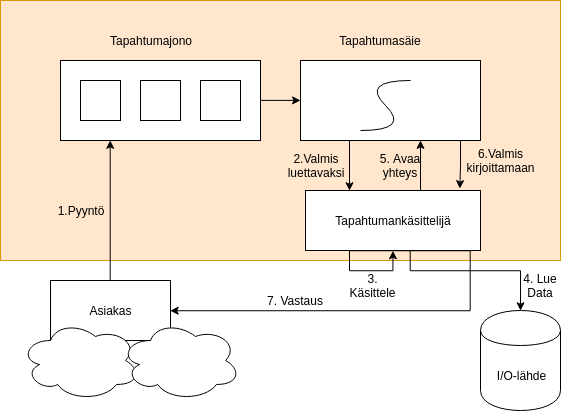
\includegraphics[scale=0.5]{reactor.png}
\end{figure}

Mallin tapahtumakäsittelijöissä rinnakkaisuuteen päästään
vain I/O:n osalta, kun käytetään asynkronisia
I/O-operaatiota.
Estäviä operaatioita tulee välttää,
sillä niiden käyttäminen laskee sovelluksen
vastaavuutta huomattavasti~\cite{schmidt_reactor:_1995}.
Asynkronisia I/O-operaatioita
voidaan suorittaa niitä tarjoavien käyttöjärjestelmä kutsujen
avulla, tai siirtämällä I/O-operaatiot toisen säikeen tehtäväksi.
Itse Reactor-malli ei ota kantaa miten asynkroninen operaatio toteutetaan.
Jos tapahtumakäsittelijässä tarvitaan pitkäkestoista laskentaa
kannattaa sitä varten luoda uusi prosessi tai säie. Tämä
prosessi tai säie saattaa pyynnön loppuun rinnakkain
tapahtumasäikeen kanssa~\cite{schmidt_reactor:_1995}.

Reactor-malli on osa Proactor-mallia.
Siinä hyödynnetään käyttöjärjestelmän asynkronisia ominaisuuksia suorittamaan
operaatiota ennen pyynnön saapumista tapahtumasäikeelle~\cite{pyarali_proactor_1997}.
Reactor-mallinen osa ohjaa tässä mallissa asynkronisten tapahtumien
valmistumistapahtumia niitä vastaaville tapahtumankäsittelijöille~\cite{pyarali_proactor_1997}.
Proactor mallin tavoite on yksinkertaistaa asynkronisten ohjelmien kehitystä.
Proactor-mallissa voidaan suoraviivaisesti suorittaa toisistaan riippuvaisia
asynkronisia-operaatioita, asettamalla asynkronisten tapahtumien valmistumisille
käsittelijöitä.
Tätä toimintatapaa kutsutaan vastakutsuksi.
Vastakutsuja voi asettaa sisäkkäin ja näin voidaan rakentaa riippuvaisten
asynkronisten operaatioden ketjuja. Ketjuilla voidaan
rakentaa peräkkäistä I/O-logiikkaa estämättä muiden asiakkaiden
pyyntöjen käsittelyä.

Proactor-mallia suositellaan käytettäväksi, jos sovellus vaatii
asynkronisten operaatioiden kutsumista ja sovellus tarvitsee ilmoituksen
asynkronisen operaation valmistumisesta.
Pyyntöjen käsittely Proactor-mallissa käydään läpi kuvassa 2 ja
esimerkissä \autoref{esim:proactor}.
Kuva 2 noudattaa Proactorin~\cite{pyarali_proactor_1997} esittelyyn tehtyä
kuvaa, jossa Proactor-palvelin käsittelee pyynnön, mutta kuvassa 2
korostetaan Proactoriin-sisältyvää Reactor-mallia.
\begin{figure}
  \caption{Pyynnön käsittely Proactor-mallissa~\cite{pyarali_proactor_1997}}
  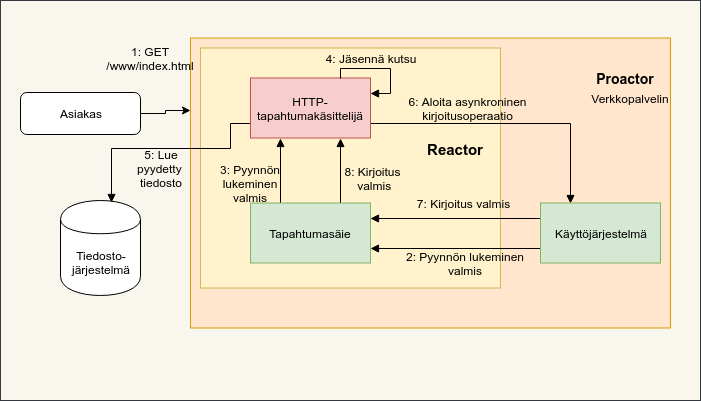
\includegraphics[scale=0.5]{Proactor.png}
\end{figure}

% ESIMERKIN LAINAAMINEN
\begin{center}
  \begin{esim}\label{esim:proactor}
    Pyynnön käsittely Proactor-mallisessa palvelimessa~\cite{pyarali_proactor_1997} \\
    \begin{enumerate}
      \item Asiakas lähettää HTTP GET pyynnön.
      \item Käyttöjärjestelmä lukee pyyntöä sovittuun puskuriin ja ilmoittaa kun valmis.
      \item Valmistumisohjaaja (Reactor) kutsuu HTTP-tapahtumakäsittelijää.
        Kohdat 2 ja 3 toistuu kunnes koko pyyntö on luettu.
      \item HTTP-tapahtumakäsittelijä jäsentää kutsun.
      \item HTTP-tapahtumakäsittelijä lukee pyydetyn tiedoston.
      \item HTTP-tapahtumankäsittelijä aloittaa asynkronisen operaation
        kirjoittaakseen tiedoston datan asiakasyhteyteen, ja asettaa
        itsensä tapahtumakäsittelijäksi kirjoituksen valmistumiselle.
      \item Kun kirjoitusoperaatio on valmis käyttöjärjestelmä ilmoittaa
        Valmistumisohjaajalle.
      \item Valmistumisohjaaja huomauttaa HTTP-tapahtumakäsittelijää,
        koska se asetti itsensä tapahtumankäsittelijäksi kirjoituksen
        valmistumiselle. Kohtia 6 - 8 toistetaan kunnes koko tiedosto on lähetetty.
    \end{enumerate}
  \end{esim}
\end{center}
Niin kuin Reactor-malli, Proactor ei myöskään sovellu laskennan samanaikaistamiseen.
Proactorin muutokset rajoittuvat asynkronisten-operaatioden ohjaamisen
kehittämiseen. Mallissa tapahtumasäie kutsuu tapahtumankäsittelijöitä, jolloin
pitkäkestoisen laskennan suorittaminen tapahtumankäsittelijässä, johtaisi
muiden pyyntöjen odotusajan kasvuun. Malliin pitää siis
lisätä muita mekanismeja laskennan rinnakkaistamiseksi.

Modernissa verkkopalvelinsovelluksessa Proactor-mallin suosioon on
monta syytä. RESTful-rajapinnan käyttäminen
verkkopalvelinsovelluksessa viestien välitykseen,
saa viestien koon pysymään pienenä ja viestien
käsittelyyn kuluvan ajan lyhyempänä verrattuna
HTML-tiedosto vastaukseen[lähde?]. % Etsi joku REST-lähde
Monisäikeisyys ja rinnakkaistaminen
voidaan järjestelmän arkkitehtuurissa siirtää tietokantamoottorin vastuulle,
jolloin verkkopalvelin voi lähettää sille asynkronisia kyselyitä
ja näin suorittaa useisiin pyyntöihin liittyviä tietokantakyselyitä
samanaikaisesti. Tämä vaatii Proactor-mallin sillä asynkronisen tietokantaoperaatioon
pitää kytkeä vastakutsu tiedon käsittelyyn ja lähettämiseen.
Tämänkaltaisella toteutuksella verkkopalvelimen käyttötapaus sopii
hyvin yhteen Proactor-mallin määrittelyn kanssa tukeutuen
mallin vahvuuksiin sekä peittäen sen heikkouksia.



Toinen Reactor mallin laajennus on SEDA (Staged Event Driven Architecture)~\cite{welsh_seda_2001}.
Siinä pyyntöjen käsittely jaetaan tasoiksi, joissa kaikissa on
käytännössä reactor-mallin toteuttava rakenne. Jokaisella tasolla
on oma tapahtumajono sekä tapahtumakäsittelijä, joka ohjaa työtä
apusäikeille. Tasoilla ei ole tapahtumasäiettä, sillä
jokaisella tasolla on vain yksi tapahtumakäsittelijä.
Tapahtumakäsittelijä voi käsittelyn päätteeksi
lisätä uusia tapahtumia seuraavien tasojen tapahtumajonoihin.
Tämän lisäksi jokaisella tasolla on resurssiohjaaja,
joka vastaa resurssien käytön pysymisestä sallitulla tasolla,
sekä apusäikeiden määrästä kyseisellä tasolla~\cite{welsh_seda_2001}.
SEDA-arkkitehtuurin suurin ero suoraan Reactor-mallin pohjalta luotuun
palvelimeen on sen hienojakoisempi resurssien ohjaus sovelluksen eri tasoille.
SEDA-arkkitehtuurilla on mahdollista myös saavuttaa rinnakkaisuutta
laskennallisesti vaativissa tehtävissä.

Tässä tutkielmassa keskitytään erityisesti
Proactor-malliin, sillä se on sisäänrakennettu Node.js ohjelmaympäristöön ja
täten paljon käytetty. Node.js:n Proactor-mallin toteuttamisesta vastaa
libuv-kirjasto~\cite{libuv_design_2019}. Suunnittelufilosofiassa
libuv:lla on paljon yhteistä AMPED-mallin kanssa, sillä
sen tarkoitus on taata aina asynkroniset I/O-operaatiot alustasta
riippumatta. Libuv siirtääkin I/O-kutsun toiselle säikeelle
jos alustalla ei ole tarjota asynkronista kutsua~\cite{libuv_design_2019}.
Tämä toimintapa saa kutsun näyttämään tapahtumankäsittelijästä
asynkroniselta.

Reactor-mallia voi laajentaa vielä kolmannella tavalla.
Jos samaa Reactor-sovellusta ajaa yhdessä eri säikeillä tai prosesseilla
ja jokin säie jakaa työn tasaisesti tapahtumasäikeiden välillä
on kyseessä SYMPED-malli. Tämä malli mahdollistaa
Reactor pohjaisten sovelluksien skaalaamisen tehokkaasti.

\subsection{Säiereservimalli}
Monisäikeisiä palvelinmalleja on useita, mutta tässä tutkielmassa keskitytään säiereservimalliin.
Monisäikeiset mallit ovat käytännössä syrjäyttäneet moniprosessimallin,
sillä palvelimien käyttöjärjestelmät tukevat säikeitä, ja säikeiden hallinnointiin
kuluu vähemmän resursseja kuin prosessien ja niiden välinen kommunikointi on sujuvampaa.
Moniprosessimallia käytetään kuitenkin yhä, kun järjestelmä pitää
saada skaalautumaan usealle laitteistolle.

Monisäikeisissä palvelinsovelluksissa hyödynnetään laitteiston
rinnakkaisuutta tehokkaasti suorittamalla pyyntöjä usealla säikeellä rinnakkain.
Suunnittelun keskeisenä tavoitteena on käsitellä mahdollisimman monta pyyntöä rinnakkain ja
näin saavuttaa korkea volyymi. Mallin suorituskyky voi kuitenkin
kärsiä synkronointiin ja säikeiden hallinnointiin kuluvasta
suoritinajasta~\cite{pyarali_proactor_1997}.

Pääsääntöisesti nämä mallit skaalautuvat hyvin laitteistoresursseihin,
mutta jos hallinnoitavien säikeiden määrä on huomattavasti suurempi kuin laitteiston
fyysisten suorittimien määrä, aiheuttaa hallinnointi ylimääräistä taakkaa.
Kalleimmat hallinnointitehtävät ovat säikeiden luonti ja tuhoaminen, sillä
muistin varaus- ja vapautusoperaatiot vievät paljon aikaa~\cite{ling_analysis_2000}.
Näihin operaatioihin kuluva aika onkin suurin säie-yhteyttä-kohti mallin
ongelma, jossa jokaista asiakas yhteyttä kohti
luodaan uusi säie, joka vastaamisen jälkeen tuhotaan.
Tämän mallin ongelmia on pyritty ratkaisemaan säiereservimallilla.

Säiereservimalli pyrkii minimoimaan tämän ongelman rajoittamalla
säikeiden määrän johonkin järkevään arvoon, kuten fyysisten suorittimien
määrään. Se käyttää samoja säikeitä uudestaan, eli se ei tuhoa säiettä
pyynnön käsittelyn päätteeksi vaan jättää sen vapaaksi säikeeksi reserviin~\cite{ling_analysis_2000}. Rajattu säikeiden määrä saattaa kuitenkin aiheuttaa epäreiluutta
pyyntöjen käsittelyyn, jos kaikki säikeet ovat jo käytössä pyynnön
saapuessa palvelimelle. Tämä voi aiheuttaa yksittäiselle asiakkaalle
huomattavan suuren viiveen~\cite{welsh_seda_2001}.

Säiereservimallissa asiakkaan pyyntöjen käsittely tapahtuu seuraavasti.
Kun pyyntö saapuu, se osoitetaan vapaalle säikeelle. Säie käsittelee pyyntöä ja,
jos se jää odottamaan I/O:ta asetetaan säikeen tila suorittaa-tilasta odottaa-tilaan,
jolloin käyttöjärjestelmän vuoronantaja voi antaa suoritinaikaa toiselle säikeelle,
kunnes I/O-pyyntö valmistuu. Kun pyyntö on käsitelty ja siihen on vastattu, niin
säie siirretään takaisin reserviin~\cite{ling_analysis_2000}.

Menetelmässä pyyntöjen käsittely on hyvin eristetty toisistaan ja
yhden säikeen lukittava tapahtuma ei vaikuta muihin säikeisiin negatiivisesti~\cite{davis_case_2017}.
Tämä edistää monisäikeisen mallin vakautta ja kykyä vastustaa hyökkäyksiä.
Tämä malli on myös ohjelmoijalle yksinkertainen sillä, pyyntöjen jakamaa tilatietoa
ja synkronointia on vähän~\cite{hu_applying_1998}.

Säiereservin oikean kapasiteetin valitseminen on erittäin kriittinen
järjestelmän suorituskyvylle.
Väärin valittu reservin koko kumoaa kaiken hyödyn, mitä luomisoperaatioiden
ja tuhoamisoperaatioiden välttämisellä on saavutettu~\cite{ling_analysis_2000}.

Joissain toteutuksissa kokoa voi myös muuttaa dynaamisesti ajon aikana vastaamaan
reaaliaikaiseen tarpeeseen.
Tunnettuja säiereservimallin toteutuksia ovat MySQL, sekä Apache Tomcat.

SYMPED-malli ja säiereservimalli ovat samankaltaisia ja SYMPED onkin
säiereservimallin erikoistapaus, joissa jokainen reservin säie on
Reactor/Proactor mallinen palvelin,
joiden välillä työ jaetaan.

\section{Mallien vertailu ja analyysi}
Seuraavaksi esitellään arviointikriteerit,
joilla malleja vertaillaan.
Vertailu perustuu aiempaan kirjallisuuteen, niissä
tehtyihin testeihin ja arvioihin
mallien soveltuvuudesta eri
käyttötapauksiin.
Vertailua ohjaava ajatus on:
edistääkö mallin käyttäminen palvelimen
suorituskykyä rinnakkaisuutta kasvattamalla
nostamatta sovelluslogiikan kehitystyön haastavuutta
sietämättömälle tasolle.

\subsection{Arviontikriteerit}
Palvelimen roolin kannalta olisi toivottavaa, että
se pystyisi käsittelemään mahdollisimman paljon pyyntöjä
ajan yksikössä. Sen tulisi pystyä myös käsittelemään pyyntöjä
luotettavasti eli lopulta kaikki pyynnöt käsitellään ja niihin vastataan.
Yksittäiselle asiakkaalle tärkein suorituskyvyn mittari on se kuinka kauan
yksittäiseen pyyntöön vastaaminen vie. Pyynnön matala vasteaika saa
palvelun käyttökokemuksen tuntumaan sujuvammalta.
Skaalautuvuus on tärkeää palvelinta ylläpitävälle taholle, sillä
näin käyttäjämäärän kasvaessa voidaan suorituskykyä parantaa
lisäämällä laitteistoresursseja. Järjestelmän tulisi myös
olla vastustuskykyinen hyökkäyksille.
Verkkopalvelimen samanaikaistamiskäytännön tulisi
yksinkertaistaa samanaikaisuuden hallintaa sovelluksessa~\cite{pyarali_proactor_1997}.
Kehitystyön helpottaminen vähentää kustannuksia
järjestelmän, kun järjestelmää rakennetaan, laajennetaan ja ylläpidetään.
Siksi järjestelmän rakenteen yksinkertaisuus ja
ymmärrettävyys on haluttava ominaisuus.
Näin on valittu seuraavat kriteerit
järjestelmien vertailuun.
\begin{itemize}
  \item käsiteltyjen pyyntöjen määrä eli volyymi
  \item menetysprosentti
  \item skaalautuvuus laitteistoresursseihin
  \item vasteaika
  \item vakaus
  \item kehitystyön haastavuus
\end{itemize}

\subsection{Järjestelmien volyymin ja skaalautuvuuden testit simulaatiolla}
Vuonna 1997 James C. Hu et.al testeissään~\cite{hu_measuring_1997}huomasivat
että pienillä tiedostoilla säiereservimalli oli paras,
mutta suuremmilla tiedostoilla asynkroninen I/O-operaatioiden
tekeminen tapahtumaohjatulla palvelimella oli kaikista tehokkain.
Testissä asynkronisia operaatioita hidasti
erityisesti TransmitFile-funktio, joka oli
hidas pienillä tiedostoilla.
Tästä tuloksesta voidaan kuitenkin huomata,
että suurilla tiedostoilla saadaan asynkronisilla
kutsuilla aikaan enemmän I/O:n rinnakkaisuutta, sillä
työ siirtyy käyttöjärjestelmän vastuulle.

TransmitFile-funktio aiheutti pienillä 500-tavuisilla tiedostoilla hyvin suuren viiveen
pyynnöille, joka oli noin 200ms. Samalla tiedostokoolla säiereservimallin palvelin
suoriutui vain noin 50ms viiveellä. Menetelmien asetelma vaihtaa paikkaa
50K-kokoisilla tiedostoilla, joilla Asynkronisia kutsuja käyttävän
palvelimen viive laski alle säiereservimallin arvon. Suuremmilla tiedostoilla
ero korostui entisestään. Pienillä tiedostoilla säiereservimallilla oli suurempi
volyymi, mutta myös tämä tilanne kääntyi tiedostokoon kasvaessa.


Ivan Voras ja Mario Zagar testasivat~\cite{voras_characteristics_2009},
verkkopalvelimen rinnakkaistamismalleja mdcached keskusmuistitietokannan
käyttötapauksessa. Käyttötapauksen erikoispiirre on että, siihen ei liity levy I/O:ta
vaan järjestelmän suorituskyky on pääasiassa riippuvainen muistiväylän nopeudesta sekä
käyttöjärjestelmäkutsujen nopeudesta.

Järjestelmistä mitattiin operaatioiden (transaction) määrä sekunnissa vaihtuvilla tietyillä
asiakasmäärillä. Kaikki mallit testattiin samalla laitteistolla.

Testissä he huomasivat,
että heidän SEDA-implementaationsa kahdella tapahtumasäikeellä ja 4 apusäikeellä
ei saavuttanut huomattavaa
etua yksinkertaiseen Reactor-toteutukseen. Tämän diagnosoitiin
johtuvan SEDA:n aiheuttamien suoritinympäristön vaihtojen yleisyydestä
sekä säikeiden välisestä kommunikoinnista.
Testissä molemmat järjestelmien suorituskyky
oli lähes samalla 120:een asiakkaaseen asti jonka
jälkeen SPED-järjestelmän suorituskyky alkoi
hieman heikentyä. SPED suoritti silloin noin 110 000 toimitusta sekunnissa
ja SEDA 120 000 sekunnissa.

SEDA-mallissa jokaisella käsittelyn vaiheella on omat apusäikeensä,
joilla saadaan rinnakkaistettua vaiheeseen liittyvää estävää laskentaa.
Muistitietokannan käyttötapauksessa estävää laskentaa on vähäisesti.
Kuitenkin vaiheesta toiseen siirtyminen aiheuttaa suoritinympäristön vaihdon,
kun uuden vaiheen apusäie otetaan käyttöön.
Apusäikeiden hyödyt
tulisivat näkyviin selkeämmin käyttötapauksessa, jossa vaaditaan enemmän
rinnakkaista estävää laskentaa, kun Muistitietokannan tapauksessa.

Samassa testissä AMPED-järjestelmä neljällä apuprosessilla
kykeni 250 000 toimitukseen sekunnissa 120:nellä asiakkaalla. Mielenkiintoista on
että heidän SEDA-implementaatio, jossa tapahtumasäikeiden ja apusäikeiden
määrät asetettiin samaksi arvoksi suoritui huomattavasti paremmin ja
saavutti 300 000 tapahtumaa sekunnissa 120:nellä asiakkaalla.
Vertailun selkein voittaja skaalautuvuuden
osalla oli SYMPED-järjestelmä, jossa on useita SPED-järjestelmiä
omilla säikeillään. Tällä järjestelmällä neljällä säikeellä
saavutettiin 440 toimitusta sekunnissa 120:nellä asiakkaalla.
SYMPED-järjestelmä osoitti myös hyvää skaalautuvuutta
sille annettujen säikeiden määrän kasvaessa.


\subsection{Sovelluslogiikan kehitystyön haastavuus}
Rinnakkaistamisen toteutusmallit ovat työkaluja kehittäjälle,
jotka toteutetaan mielekkäästi kirjastona tai moduulina.
Jos malli on hyvin toteutettu kehittäjän tulisi pystyä
keskittymään keskeisen sovelluslogiikan kirjoittamiseen
murehtimatta rinnakkaisuutta hallitsevasta osasta.

Reactor-malli on yksinkertainen ja helpommin toteutettava
kuin Proactor. Reactor-mallin onnistuu hyvin tavoitteessaan
erottaa pyyntöjen samanaikaistamiseen liittyvä logiikka
muusta sovelluslogiikasta.
Tapahtumaohjatut sovellukset tuovat omat haasteensa
ohjelmoijalle, sillä niistä virheiden löytäminen ja
korjaaminen on usein työlästä, koska ohjelman
suoritus ei kulje rivi riviltä, vaan järjestys
muuttuu tapahtumakäsittelijöiden ja vastakutsujen mukaan.

Reactor-mallia käyttävässä palvelimessa kehittäjän
pitää huolehtia siitä, että yksittäisen pyynnön
käsittelyyn menee vähän aikaa~\cite{pyarali_proactor_1997}, koska
tapahtumasäikeen aika pitää jakaa tehokkaasti
kaikkien pyyntöjen välillä. Tämä mahdollistetaan
vain vähälogiikkaisilla tapahtumankäsittelijöillä, sekä
asynkronisilla I/O-kutsuilla.

Reactor-mallin toteutuksissa kehittäjän tulee huomioida
asynkronisen I/O:n vaikutukset. Asynkronisuus vaikeuttaa koodin
luettavuutta, mutta se nostaa ohjelman samanaikaisuutta ja täten
tehokkuutta huomattavasti. Sovelluslogiikan kehittäjän
tulee myös huolehtia, että kirjoitettava logiikka
käyttää asynkronisia kutsuja~\cite{pyarali_proactor_1997}, sillä estävät
kutsut pysäyttävät koko sovelluksen suorituksen.

Ongelmana on myös pidetty käyttöjärjestelmien huonoa
tukea asynkronisille kutsuille~\cite{pyarali_proactor_1997}. Järjestelmä kutsu
$select$ johon perustui käyttöjärjestelmien Reactor-toteutuksia,
ei salli useamman säikeen odottaa saman tunnistejoukon tapahtumia.
Tämä ominaisuus estää tehokkaan laitteiston rinnakkaisuuden hyödyntämisen.
Asynkronisten kutsujen tuki on kuitenkin parantunut.
Linux-ytimen versiossa
2.4.44 siihen lisättiin $epoll$ järjestelmäkutsu~\cite{man_epoll}, joka
mahdollistaa tapahtumapohjaisen I/O:n useammalla säikeellä
samaan aikaan. BSD-ytimessä vastaava toiminnallisuus on toteutettu $kqueue$
kutsuun.
% Yritä löytää onko kutsujen ominaisuudet muuttuneet parissa kymmenessä vuodessa
Jos ohjelman tulee käsitellä
asynkronisen operaation tulosta tulee operaation valmistumiselle,
asettaa tapahtumakäsittelijä. Tätä toimintatapaa kutsutaan vastakutsuksi (callback)
Tässä tilanteessa Proactor-malli on erittäin hyödyllinen, sillä se
kuvailee selkeästi miten asynkronisten tapahtumien valmistumisia tulisi käsitellä.

Proactor-mallissa kuten Reactor-mallissa sovelluslogiikka ohjelmoidaan
tapahtumankäsittelijöihin, mutta Proactor-mallissa liittyy
mallille tyypillisesti vastakutsuja. Jos vastakutsuja ei tarvittaisi
voitaisiin vain käyttää Reactor-mallia ja unohtaa Proactor kokonaan.
Vastakutsut ovat haastava konsepti. Ne vaikeuttavat vianetsimistä
sovelluksesta, koska sovelluksen kulku vaihtelee kehysinfrastruktuurin
ja tapahtumakäsittelijöiden logiikan välillä. Täten sovelluksen
kulkua on vaikea seurata askel askeleelta.

Vastakutsujen abstraktioita ohjelmointikielissä ovat Promise, Future ja
async/await. Ne auttavat kehittäjää hahmottamaan vastakutsujen
toimintaa korkealla tasolla.

Proactor-mallissa kehittäjä on vaikeaa vaikuttaa sovelluksen
aikataulutukseen~\cite{pyarali_proactor_1997},
sillä asynkronisen operaatioiden luojalla
ei ole mahdollisuutta ohjata operaatioiden valmistumisjärjestystä.
Toteutuksen tulisikin siksi tarjota kehittäjälle mahdollisuuden
priorisoida ja keskeyttää asynkronisia operaatioita.
Jos kehittäjä olettaa asynkronisten kutsujen valmistuvan tietyssä järjestyksessä,
voi se johtaa eräänlaiseen kilpailutilanteeseen, jossa
oikea lopputulos on riippuvainen tietystä valmistumisjärjestyksestä.

Reactor-tai Proactor-mallit eivät tarjoa keinoja
laskennan rinnakkaistamiseen. Käyttötapauksissa
joissa se on tarpeen, kehittäjän tulee lisätä
mallin tapahtumakäsittelijöihin rinnakkaisuutta käsittelevää
logiikkaa kuten säikeiden luomista.


Säiereservimallissa ohjelmakoodi voidaan pitää yksinkertaisena ja
hyvin luettavana. Kehittäjät voivat vapaasti käyttää intuitiivisia
peräkkäisiä operaatioita ja estäviä kutsuja, koska sovelluslogiikkaa
suoritetaan erillisillä säikeillä~\cite{pyarali_proactor_1997}. Estävä kutsu pysäyttää vain
sen säikeen, jonka käsittelyyn se liittyy, jolloin muiden
pyyntöjen käsittely voi jatkua esteettä.

Eri asiakkaiden pyynnöt liittyvät harvoin toisiinsa,
jolloin niiden välillä ei ole merkittävästi jaettua tilatietoa ja
synkronointia tarvitaan minimaalisesti~\cite{pyarali_proactor_1997}.
Kehittäjän tulee kuitenkin ottaa huomioon mahdolliset lukkiutumiset
tai kilpailutilanteet eri pyyntöjen käsittelyn välillä, jos
käyttötapauksessa ilmenee tarve tilatiedon jakamiselle.
Pyyntöihin liittyvä laskenta rinnakkaistuu hyvin laitteistotasolla,
kun jokainen pyyntö on käsittelyssä omalla säikeellään.

SEDA-mallissa rinnakkaisuuden hallintaa edistää,
samaa tietoa käsittelevien säikeiden eristäminen samalle tasolle~\cite{welsh_seda_2001}.
Samalla tasolla synkronisoiminen ja kilpailutilanteiden ratkaiseminen on
yksinkertaisempaa kuin koko sovelluksen mittakaavassa, ja
viesteihin perustuva sovelluksen kulku on helpommin seurattavissa kuin
muissa tapahtumaohjatuissa malleissa.

SYMPED-malli on rakenteeltaan monimutkainen suhteessa muihin malleihin.
Sen vahvuus kehitystyön näkökulmasta piilee kuitenkin siinä, että
jos yksiprosessisen Reactor-palvelimen skaalautuvuus ei riitä palvelemaan
järjestelmän tarpeita, voidaan järjestelmän sovelluslogiikka
sovittaa suoraviivaisesti osaksi SYMPED-järjestelmää. Molemmissa malleissa
sovelluslogiikka ohjelmoidaan tapahtumankäsittelijöihin, ja nämä voidaan siirtää
suoraan SYMPED-toteutukseen tarpeen vaatiessa.

\subsection{Vakaus}
Palvelimen vakaudella tarkoitetaan sen kykyä vastustaa hyökkäyksiä ja
virhetiloja.
Palvelimen rinnakkaisuuden toteutusmalli vaikuttaa sen vakauteen, jos asiakkaiden
pyynnöt vaikuttavat toisiinsa tai jos rinnakkaistaminen voi aiheuttaa virhetiloja kuten
lukkiutumista.

Reactor/Proactor-malliseen palvelimeen voi kohdistaa hyökkäyksiä, joilla pyritään
myrkyttämään sovelluksen tapahtumasäie. Reactor-mallin palvelin toteutuksissa
osoitepolkujen jäsentäminen on saman säikeen vastuulla kuin sovelluksen ohjaaminen.
Tämän työvaiheen takia
tapahtumasäikeen myrkyttämiseen sopivat pyynnöt,
joiden osoitepolun selvittämiseen liittyy kompleksista
säännöllisten lauseiden käsittelyä~\cite{davis_case_2017}.
Kuvassa 2 pysähdyttäisiin siis kohtaan 4: kutsun jäsentäminen, ja
kaikki muut pyynnöt joutuvat odottamaan.
Yksi pyyntö siis aiheuttaa suhteettoman suuren työtaakan
tapahtumasäikeelle, jolloin koko sovellus jää odottamaan sitä.
Hyökkääjä lähettää näitä pyyntöjä niin paljon, että sovellus
ei pysty palvelemaan sen todellisia asiakkaita. Tämä
on palvelunestohyökkäyksen erikoistapaus.

Tällaiset hyökkäykset aiheuttaisivat ongelmia myös säiereservimallia
noudattaville järjestelmille, mutta niiden pitäisi onnistua
lukitsemaan reservin jokainen säie samaan aikaan, jotta
järjestelmä ei kykenisi enää vastaamaan asiakkaiden pyyntöihin~\cite{davis_case_2017}.

Yksinkertaisessa Reactor-malliin perustuvassa palvelinsovelluksessa ei ole
riskiä kilpailutilanteille tai lukkiutumiselle, toisin kuin säiereservimallissa.
Säiereservimallissa palvelin voi lukkiutua, jos samaan aikaan käsittelyssä olevat
pyynnöt tarvitsevat samoja resursseja käsittelyn aikana. Tämä riski on otettava
huomioon järjestelmän suunnittelussa ja sovelluslogiikan kirjoittamisessa.

Säiereservimallissa kilpailutilanteiden riski on hyvin pieni, jos pyyntöjen
välillä ei ole jaettua tilatietoa. Jaetun tilatiedon kanssa voi tulla
sivuvaikutuksia, jos pyynnöillä on mahdollisuus muokata sen sisältöä.

\subsection{Johtopäätökset}

Reactor-mallin on erottaa
selkeästi pyyntöjen käsittelyn
samanaikaistamiseen liittyvän
logiikan, muusta sovelluskohtaisesta logiikasta.
Malli on myös suhteessa muihin samanaikaisuutta
käsitteleviin malleihin yksinkertainen.
Näistä syistä se on implementoitu useisiin
kirjastoihin ja saavuttanut vakaan suosion.

Reactor-mallin rajallisuudet rinnakkaisuudessa
eivät ole haitaksi, jos järjestelmässä on rinnakkaisuutta
korkeammalla tasolla. Eli
jos Reactor-mallisia palvelmia ajetaan useita rinnakkain
ja näin luodaan SYMPED-järjestelmä.

Proactor-malli laajentaa Reactor-mallia merkittävällä,
sillä sen avulla voidaan ketjuttaa asynkronisia
operaatioita vastakutsuilla. Tämä ominaisuus
tuo joustavuutta samanaikaisen sovelluslogiikan kehittämiseen.

Proactor-mallin ansiosta rinnakkaisuus
voidaan toteuttaa myös järjestelmässä alemmalla
tasolla kuten tietokantaohjelmassa.
Proactor-palvelin voi odottaa useita asynkronisia
tietokantakyselyita samalla kun, se suorittaa
muuta logiikkaa. Eli tietokantakyselyn valmistumiskäsittelijäksi
asetetaan toiminto, joka kirjoittaa vastauksen
halutussa muodossa asiakkaalle.
Todellisen rinnakkaisen työn
suorittaa tässä käyttötapauksessa tietokantaohjelma.

Proactor-malli ei paikkaa
Reactor-mallin rajallisuutta laskennan rinnakkaistamisessa,
sillä tapahtumakäsittelijöiden logiikka suoritetaan
samalla säikeellä kuin sovelluksen kulun ohjaus.
Laskennan rinnakkaistamiseksi tapahtumakäsittelijöihin
tulee lisätä säikeiden käsittelyyn liittyvää logiikkaa.
Malli ei siis vähennä laskennan rinnakkaistamiseen liittyviä
haasteita, mutta on tehokas tapahtumien ja asynkronisten
operaatioiden hallinnassa. Nämä ominaisuudet riittävät
I/O-resurssien tehokkaaseen hyödyntämiseen.

Reactor/Proactor-mallin toteuttavalla
kirjastolla voidaan kustannustehokkaasti
toteuttaa palvelin, joka kykenee suoriutumaan
tehtävistään palvelun alkutaipaleella. Jos
käyttäjä määrät kasvavat ja skaalautuvuutta
vaaditaan voidaan järjestelmä muuttaa SYMPED-järjestelmäksi
joka todetusti skaalautuu hyvin resursseihin.
Node.js sovelluksesta voi luoda SYMPED järjestelmän
cluster-kirjastolla.

Jos laskennan suorittaminen rinnakkain usealla suorittimella
on ainoa väylä riittävän suorituskyvyn saavuttamiseksi,
ovat säiereservimalli ja SEDA-malli parempia vaihtoehtoja.
Proactor palvelimien tapahtumakäsittelijöihin
voidaan ohjelmoida säikeiden käsittelyä, mutta tämä
on täysin soveluslogiikan kehittäjän vastuulla.
Tämänkaltainen menettely olisi hybridi
SEDA-mallin ja Proactor-mallin välillä, jossa
tapahtumankäsittelijällä on säiereservi, mutta tapahtumakäsittelijät
eivät välttämättä muodosta selvää tasohierarkiaa.

\section{Yhteenveto}

Tapahtumaohjattu-malli mallintaa luontevasti verkkopalvelimen
toimintaa. Reactor-malli esittää yksinkertaisen
ratkaisun useista lähteistä tulevien tapahtumien käsittelyyn.

Verkkopalvelimen yleisimmät tehtävät ovat
HTML-tiedostojen ja nykyään kasvavissa määrin
tekstimuotoisen datan lähettäminen.
Näiden tehtävien suorituskyky on
I/O-sidonnainen.
Asynkronisilla luku-ja kirjoitusoperaatioilla samanaikaisuuden hallinta
voidaan siirtää käyttöjärjestelmän vastuulle, jolloin
verkkopalvelimen tehtävien täyttämiseen Proactor-mallinen
palvelin sopii hyvin.
Se esittää sopivat laajennukset Reactor-malliin, joilla
asynkronisia operaatioita voidaan hallita joustavasti.
Sillä voidaan suorittaa muista operaatioista riippuvaisia I/O-operaatioita
samanaikaisesti, ketjuttamalla niitä takaisinkutsuilla.
Asynkronisilla operaatioilla saavutetaan korkea I/O-resurssien
käyttöaste.

Jos palvelimen tarkoitus on suorittaa enemmän laskentaa kuin
I/O-operaatioita ei Reactor-pohjainen vaihtoehto ole paras mahdollinen.
Laskentariippuvaisessa käyttötapauksessa säiereservi tai SEDA-arkkitehtuuria
noudattava toteutus takaa huomattavasti paremman suorituskyvyn kuin
Reactor-mallia noudattava.

Proactor-tai Reactor-palvelimen voi laajentaa 
usean prosessin toteutukseksi, jos skaalautuvuus
yhdellä prosessilla ei ole riittävä palvelun tarpeisiin.


\bibliographystyle{plain}
\bibliography{kandi_zot}


\end{document}
